%%%%%%%%%%%%%%%%%%%%%%%%%%%%%%%%%%%%%%%%%%%%%%%%%%%%%%%%%%%%%%%%%%%%%%%%%%%%%%%%%%
%%                               APENDICE                                      %%
%%%%%%%%%%%%%%%%%%%%%%%%%%%%%%%%%%%%%%%%%%%%%%%%%%%%%%%%%%%%%%%%%%%%%%%%%%%%%%%%%%

\chapter{Apêndice}\label{chap:appendix}
%%%%%%%%%%%%%%%%%%%%%%%%%%%%%%%%%%%%%%%%%%%%%%%%%%%%%%%%%%%%%%%%%%%%%%%%%%%%%%%%%%
\section{Bacias de convergência}
  \begin{figure}[htp]
    \centering
    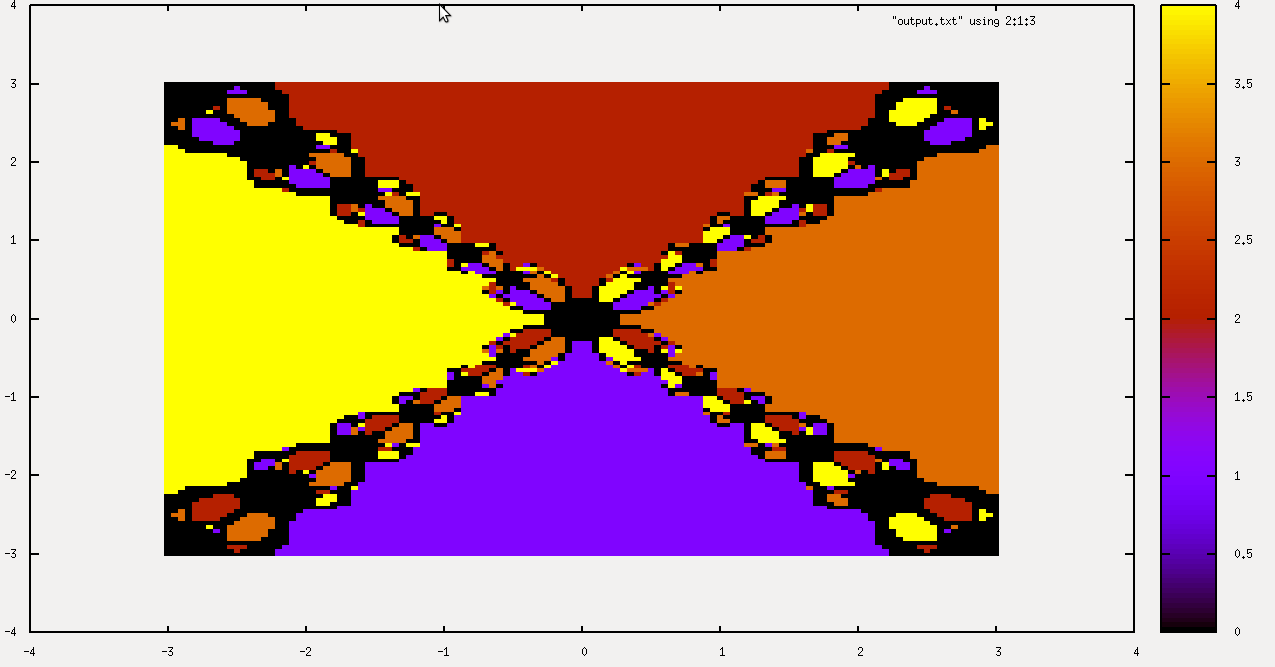
\includegraphics[width=0.9\textwidth]{imgs/img1.png}
    \caption{$f(x) = x^4 -1$ com $intervalo = [-3: 0.05: 3]$, total de 14641 pontos}
  \end{figure}

  \begin{figure}[htp]
    \centering
    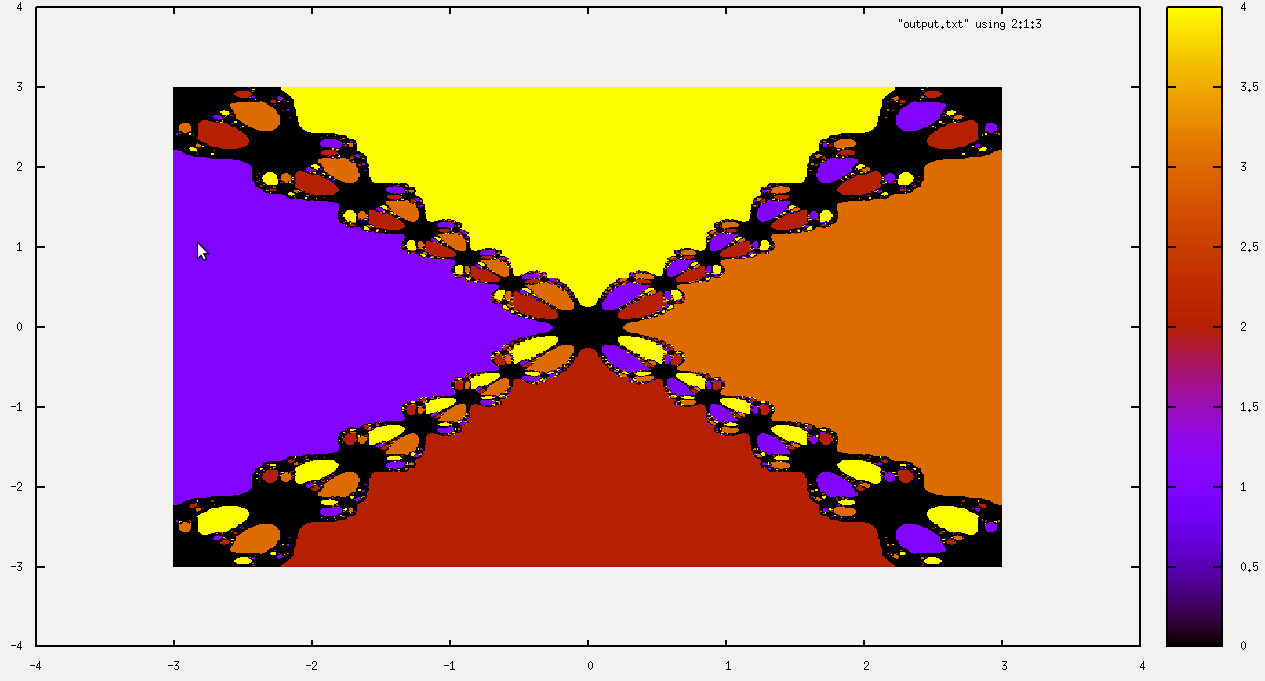
\includegraphics[width=0.9\textwidth]{imgs/img2.png}
    \caption{$f(x) = x^4 -1$ com $intervalo = [-3: 0.01: 3]$, total de 361201 pontos}
  \end{figure}

  \begin{figure}[htp]
    \centering
    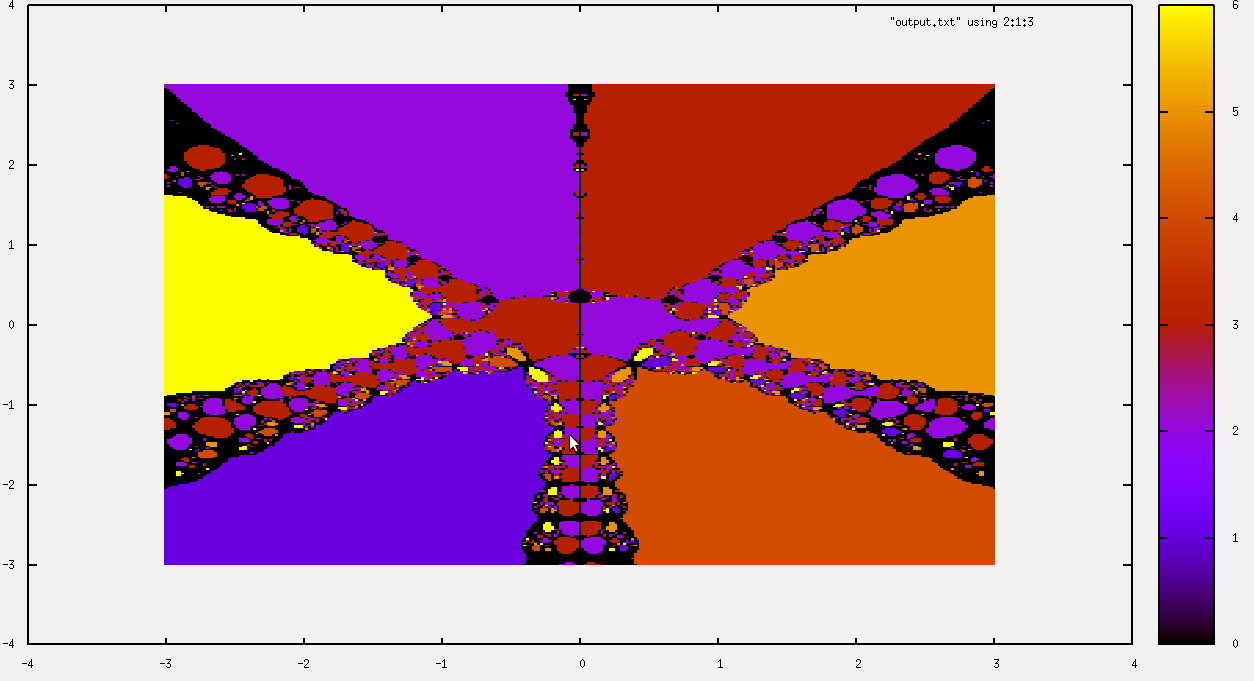
\includegraphics[width=0.9\textwidth]{imgs/img3.png}
    \caption{$f(x) = x^6 + 1*x^4 - 1*x^2 - 2*x^1 + 2$ com $intervalo = [-3: 0.02: 3]$, total de 90601 pontos}
  \end{figure}

  \begin{figure}[htp]
    \centering
    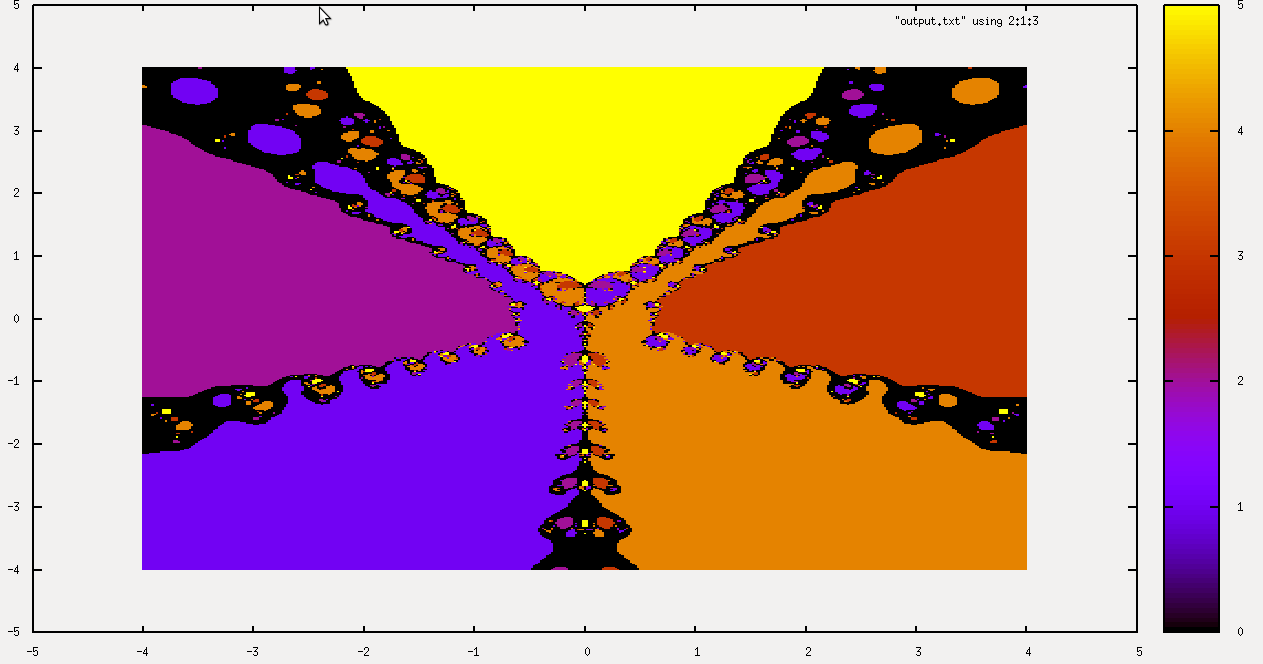
\includegraphics[width=0.9\textwidth]{imgs/img4.png}
    \caption{$f(x) = 3*x^5 + 2*x^4 + 1*x^3 - 1*x^2 - 2*x^1 - 3$ com $intervalo = [-4: 0.02: 4]$, total de 160801 pontos}
  \end{figure}

  \begin{figure}[htp]
    \centering
    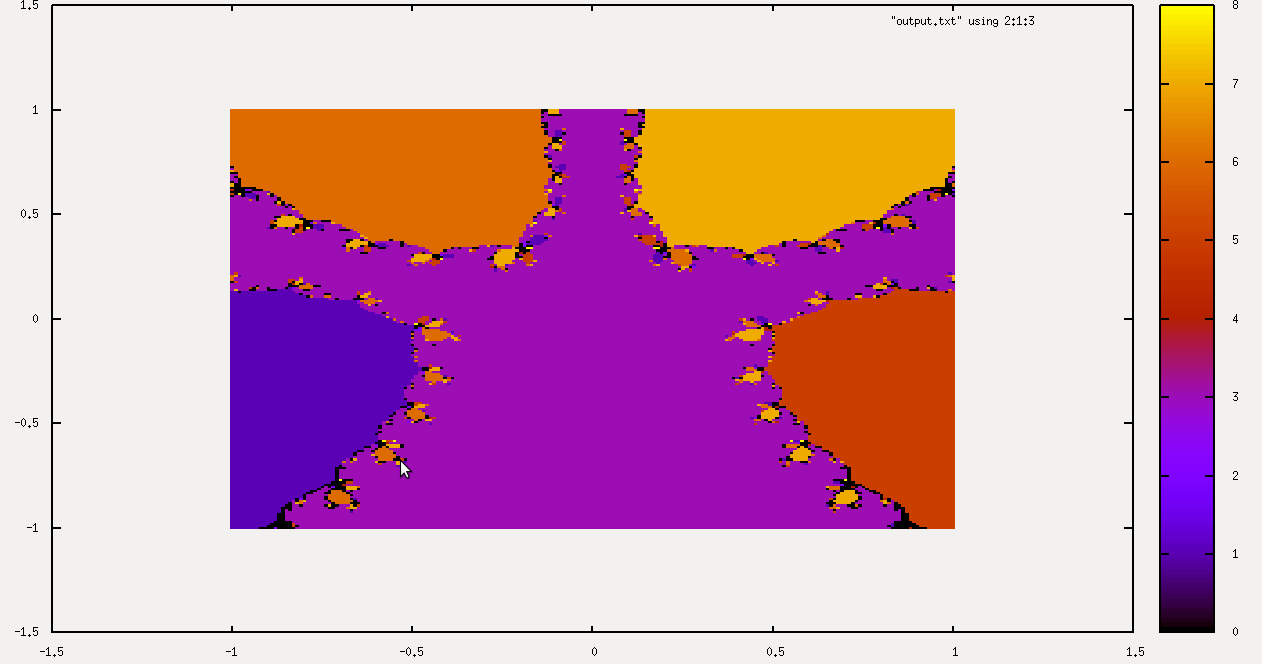
\includegraphics[width=0.9\textwidth]{imgs/img5.png}
    \caption{$f(x) = 1*x^8 + 1*x^6 + 5*x^5 - 4*x^4 + 3*x^3 - 2*x^2 + 1*x^1$ com $intervalo = [-1: 0.01: 1]$, total de 40401 pontos}
  \end{figure}

  \begin{figure}[htp]
    \centering
    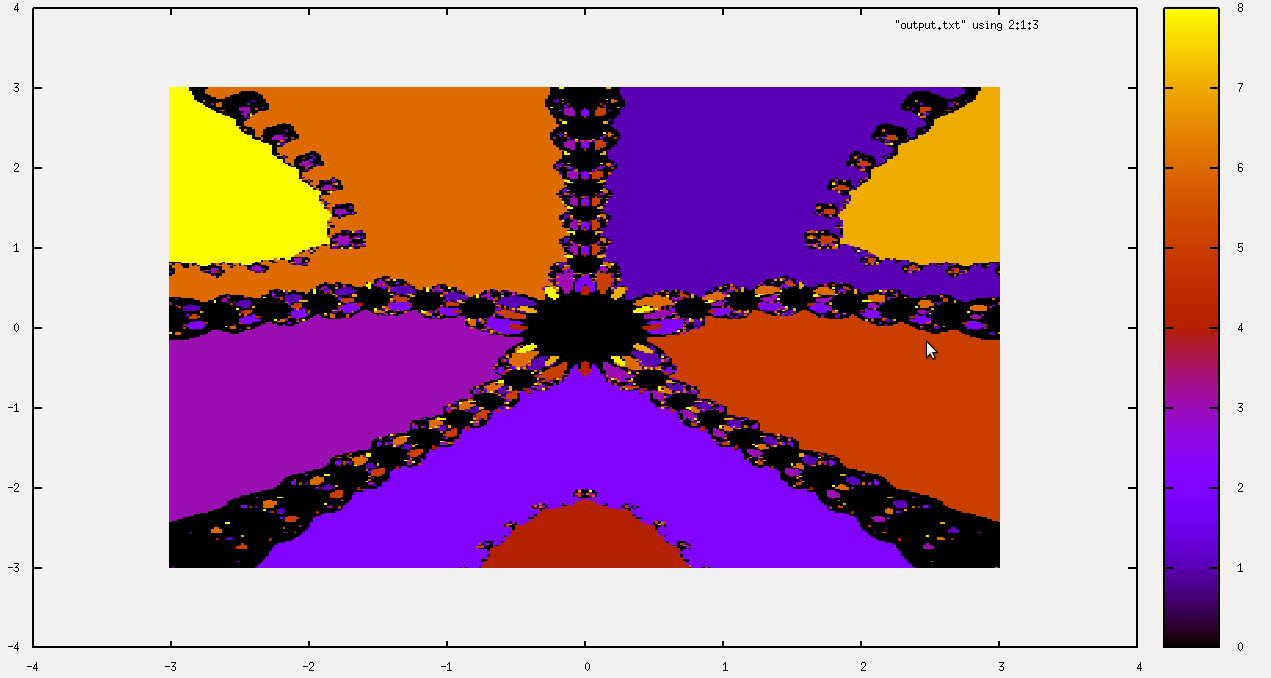
\includegraphics[width=0.9\textwidth]{imgs/img6.png}
    \caption{$f(x) = 1*x^8 + 15*x^5 + 16$ com $intervalo = [-3: 0.02: 3]$, total de 90601  pontos}
  \end{figure}